%%%%%%%%%%%%%%%%%%%%%%%%%%%%%%%%%%%%%%%%%%%%%%%%%%%%%%%%%%%%%%%%%%
\section{Introduction}\label{intro}

% Why are we studying this problem
Earthquakes can cause great damage to human society through soil
rupture, movement, tsunami, etc. Some recent earthquakes that
highlight this destructive potential are the great East Japan
Earthquake of 2011 (depicted in figure\ref{GreatEastJapan}), and the
April 2015 earthquake in Nepal. One important tool for the enactment
of policies that minimize the consequences of these events are
earthquake occurrence models (also called risk models). These models
can be used to identify patterns in the seismic mechanisms that
generate earthquakes, and are important to increase our understanding
of these events.


% \cite{ecta14} opening image. Would be better to have a clustered one.
\begin{figure}[]
\centering
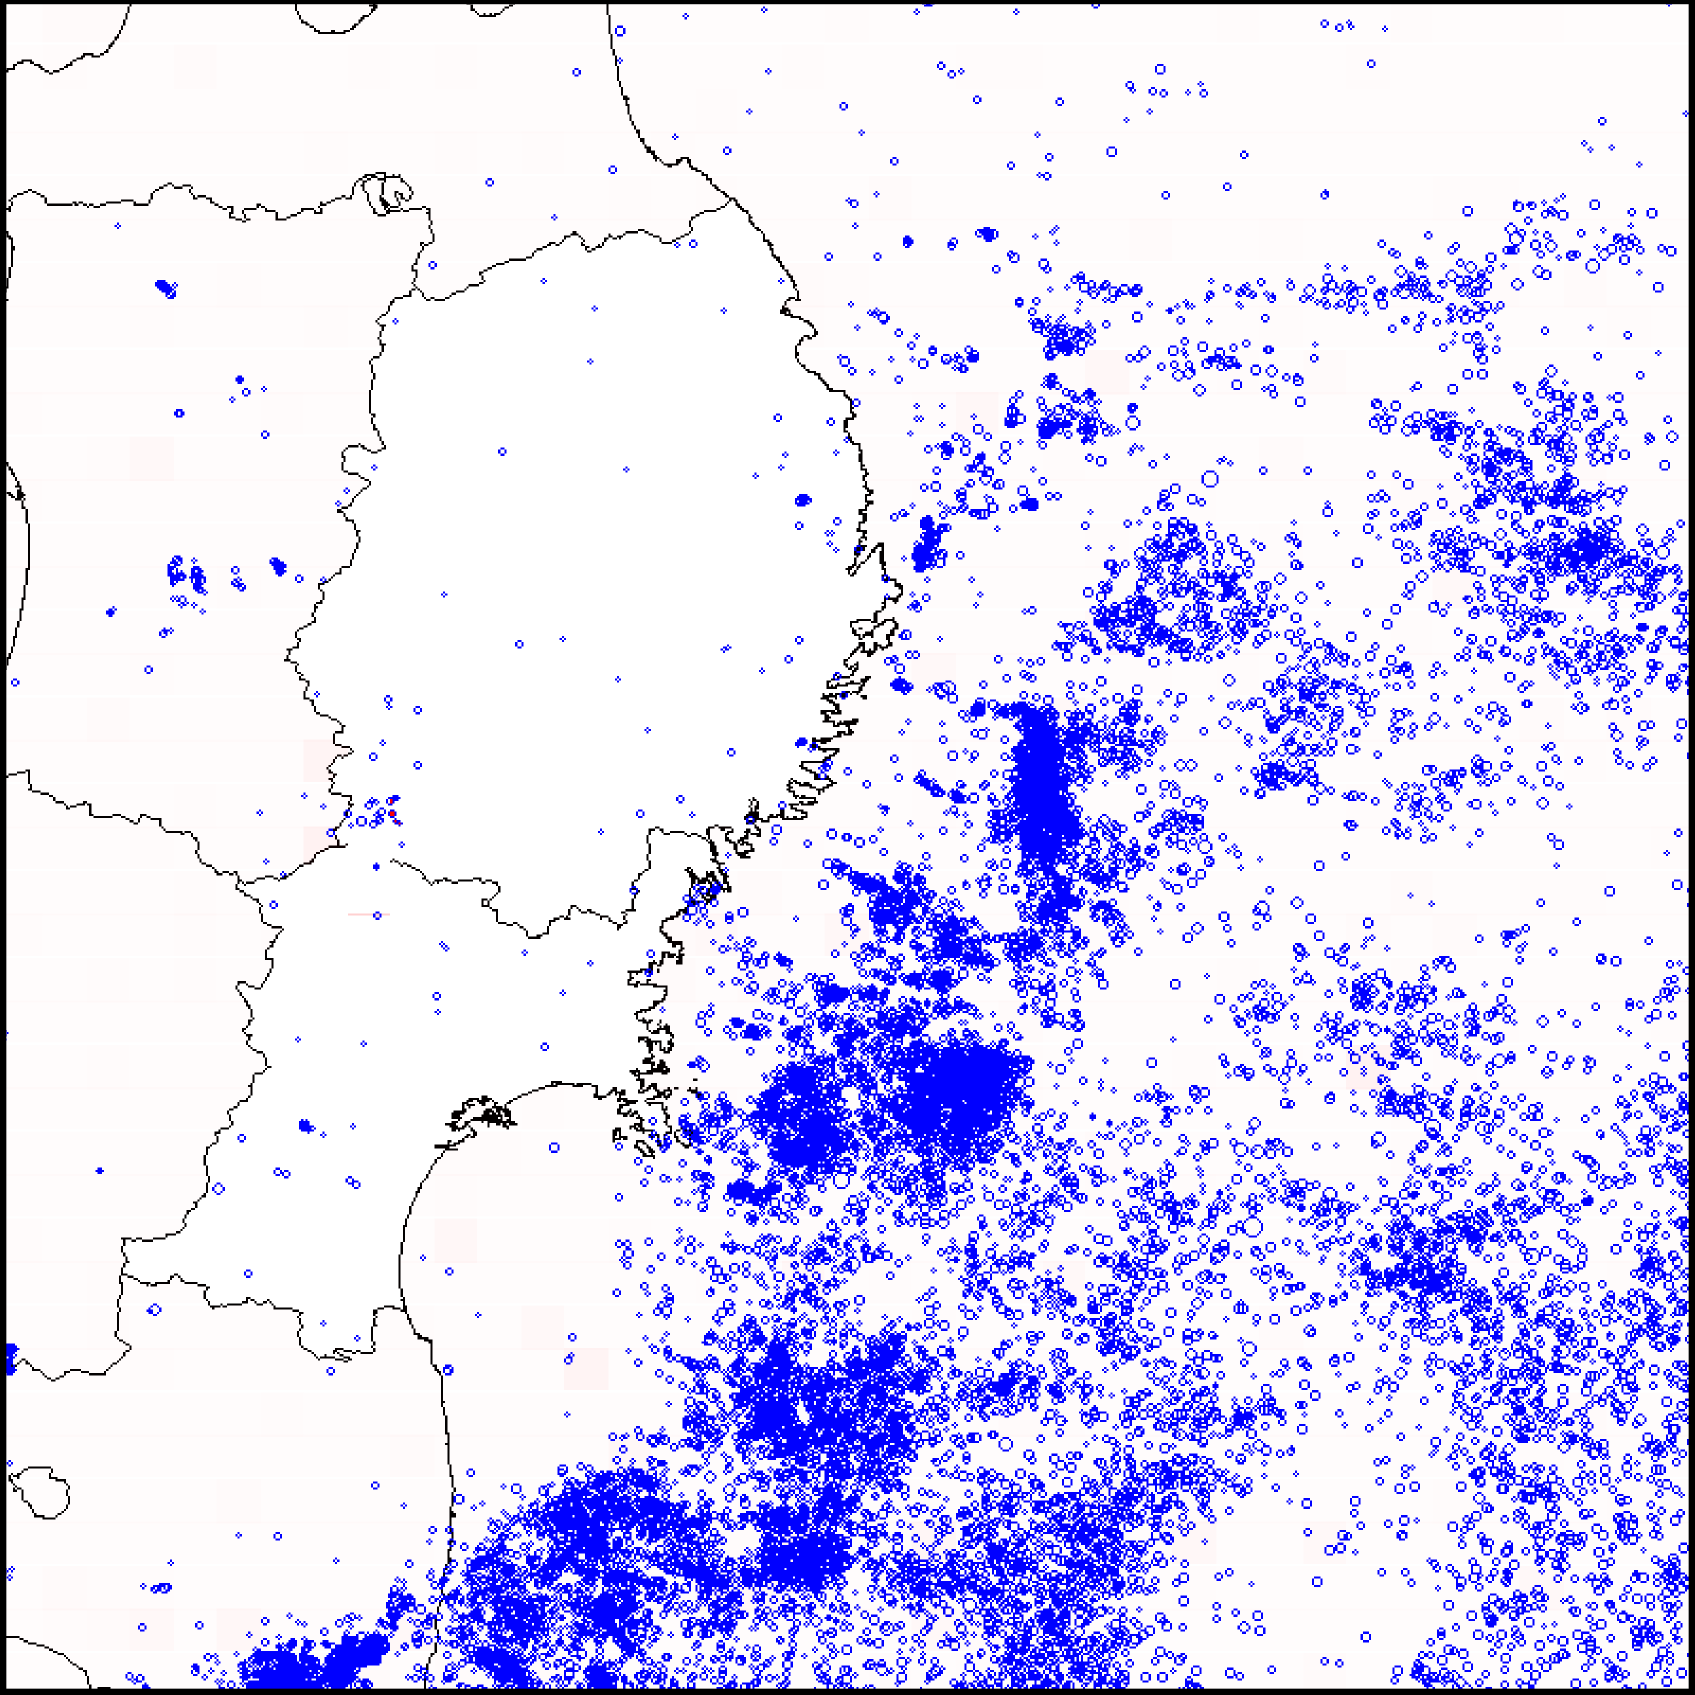
\includegraphics[width=.45\textwidth]{img/earthquakes2011.png}
\caption{Seismic Activity in Eastern Japan in 2011. Each blue dot
  represents one earthquake}
\label{GreatEastJapan}
\end{figure}

% Context of our work
In our previous work~\cite{ecta14}, we proposed a way to generate
earthquake risk models using a standard Genetic Algorithm (here called
the GAModel). The GA model was shown to be competitive with the
Relative Intensity (RI) model, while not using any a-priori
information about the distribution of earthquake occurrences (See
section~\ref{sec:background} for a summary of the GAModel, along with
other relevant literature).

In this paper, we identify three key issues with the GAModel, and
propose adjustments to the algorithms that address these issues.

The first issue is that the genome representation used by GAModel has
too many parameters (over 2000 for regular cases). Even though a
majority of these parameters do not contribute for the accuracy of the
final risk model, the size of the search space implies a slower
optimization time. To address this issue, we propose a new genome
representation for an earthquake risk model, which we will call
``Reduced Representation''. In the Reduced Representation, we avoid
representing every single location in the area under study, and only
those locations with a minimal probability of earthquake are
represented as parameters in the evolutionary process. By reducing the
search space, this representation is expected to also increase the
convergence speed of the evolutionary optimization process.

% Second issue: Hybridization with domain knowledge
The second issue is that GAModel does not take into account any sort
of domain knowledge, such as the assumption that earthquakes cluster
in both time and space. Heuristic search methods such as Genetic
Algorithms usually benefit from the introduction of domain knowledge
to the search. Therefore, we propose a hybrid version of the GAModel
which incorporates seismic models of earthquake decay. This version
generates a model with a much smaller number of earthquakes than the
regular GAModel. For each earthquake in this model, a sequence of
aftershocks is generated using an adaptation of the Epidemic Type
Aftershock Sequence model (ETAS). We expect that this hybrid approach
will produce more accurate models.

The third issue is the examination of ``de-clustering'' effects in the
historical catalog used for generating the risk model. In seismology,
de-clustering refers to the act of identifying earthquakes as either
main-shocks or aftershocks, and removing all but the main shocks from
the catalog, which is considered the representative earthquake for the
group. Accordingly, a de-clustered earthquake catalog is considered to
be easier to study, given that the de-clustering process removes
redundant information~\cite{van2012seismicity}. In this work, we
generate the de-clustered catalog by grouping earthquakes in space and
time using spectral clustering~\cite{spectral_tutorial}.

These adaptions are described in detail in
section~\ref{sec:adaptations}. We compare the contributions of each
adaptation to the generation of models based on the earthquake catalog
of the Japanese arquipelago, between 2000 and 2010. The set up of this
experiment is described in section~\ref{sec:experiment},
and the main results are listed in section~\ref{sec:results}.

Our results indicate that clustering the earthquake catalog resulted
in a significant improvement to the precision of the models
generated. On the other hand, the new representation and the
hybridization did not seem to improve the results of our models. We
discuss the implications of these findings in
section~\ref{sec:discussion}.

